Polysomnography is the gold standard method used to investigate the complexity of sleep physiology. It consists of a combination of electroencephalography (EEG), electrooculography (EOG), and electromyography (EMG) recordings from electrodes attached to the scalp, beside the eyes, and on the chin, respectively \parencite{iber_aasm_2007}. Polysomnography recordings in humans have revealed that sleep is not uniform but consists of distinct physiological stages characterised by different oscillatory patterns (Figure \ref{fig:SleepPhysio}).

\vspace{1cm}
\begin{figure}[H]
    \centering
    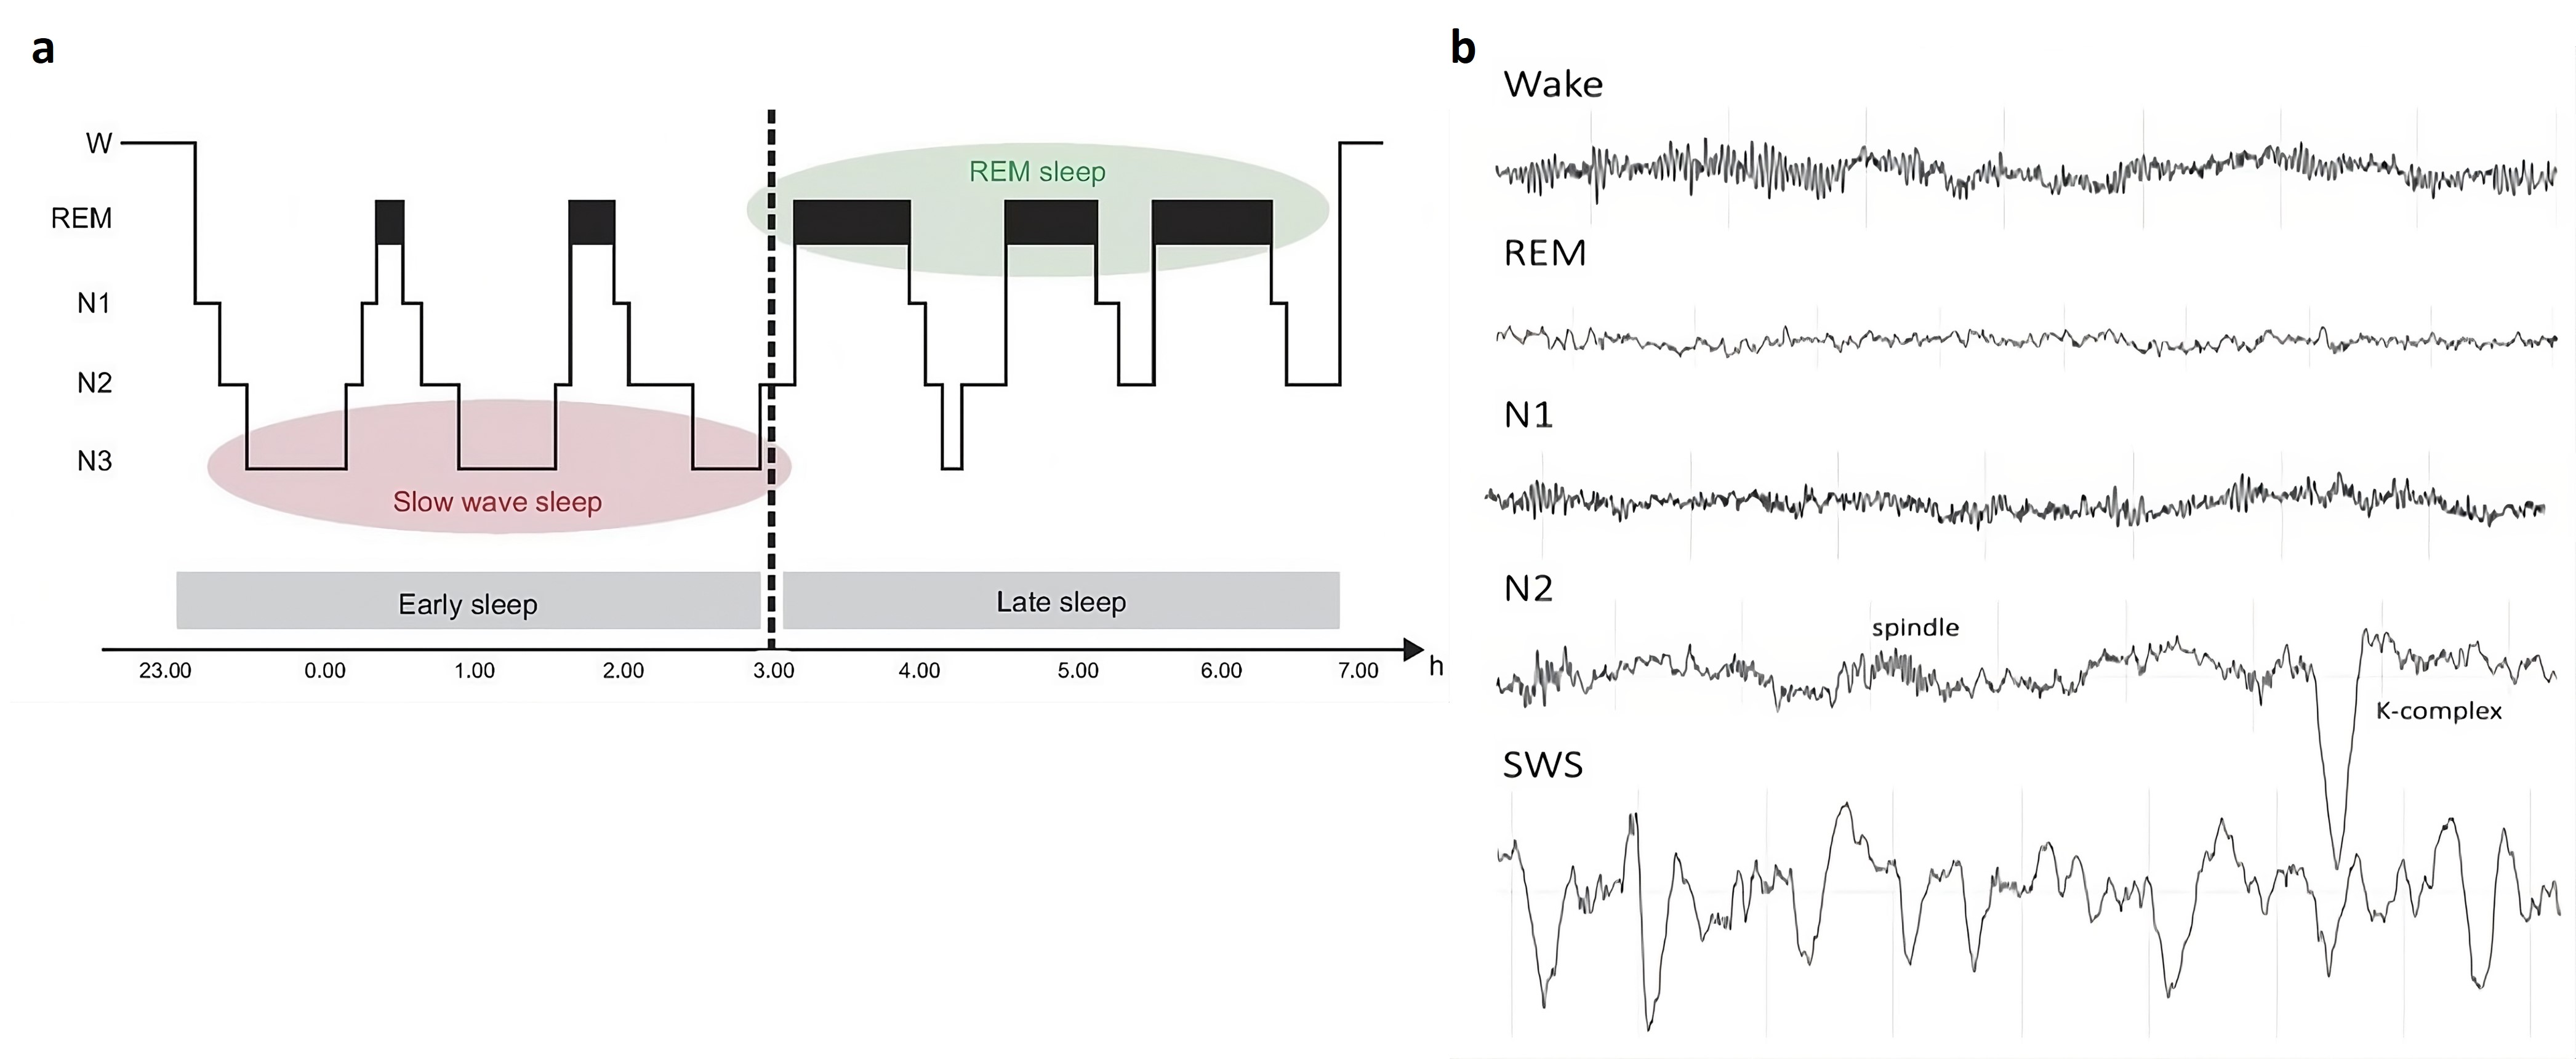
\includegraphics[width=0.9\linewidth]{1_Introduction/IntroImages/Picture1.jpg}
    \caption[\textit{Sleep architecture and oscillatory patterns.}]{\textit{Sleep architecture and oscillatory patterns.} \textbf{(a)} Hypnogram. Human sleep alternates in cycles between non-rapid eye movement (NREM) sleep and rapid eye movement (REM) sleep. Stages 3 and 4 of NREM are jointly referred to as slow wave sleep (SWS). Earlier periods of sleep are rich in SWS, whereas later periods contain greater amounts of REM sleep. Figure adapted from \cite{rasch_about_2013}. \textbf{(b)} Exemplary EEG traces for wake and each of the sleep stages. K-complexes and sleep spindles are key features of stage 2 of NREM sleep, while slow oscillations and delta waves prevail during SWS. \vspace{1cm} \label{fig:SleepPhysio}}
\end{figure}
 \FloatBarrier

The two major sleep stages that can be distinguished are Rapid Eye Movement (REM) sleep and Non-Rapid Eye Movement (NREM) sleep. The latter can be further subdivided into four stages: the lighter sleep stages 1 and 2, and the deeper sleep stages 3 and 4, now jointly referred to as slow wave sleep \parencite[SWS;][]{iber_aasm_2007}. NREM and REM sleep alternate or “cycle” across the night approximately every 90 minutes. Within each cycle, the ratio of NREM to REM varies throughout the night: NREM sleep predominates during the first half of the night, but as the night progresses, the length of REM periods becomes longer (see hypnogram in Figure \ref{fig:SleepPhysio}a). 

When transitioning from wakefulness to sleep, people typically spend a short period in Stage 1 of NREM sleep. This stage only accounts for up to 10\% of the total sleep time (TST) and is characterised by low-amplitude mixed-frequency activity (2-7 Hz) and less than 50\% of the wake-like alpha rhythm \parencite[8-13 Hz;][]{moser_sleep_2009, silber_visual_2007}. Sharply contoured waves called vertex sharp waves and slow rolling eye movements can also be observed \parencite{silber_visual_2007}. 

Stage 1 of NREM is typically followed by Stage 2, which takes up approximately 45–55\% of the TST. As shown in Figure \ref{fig:SleepPhysio}b, sleep spindles and K-complexes are the two pronounced oscillatory events that characterise this sleep stage (however, spindles can be also found during deeper sleep stages). \\
Sleep spindles are waxing and waning bursts of high-frequency activity that last about 0.5 to 3 seconds. They are generated in the thalamic reticular nucleus and then propagated into cortical regions through thalamocortical projections \parencite{de_gennaro_sleep_2003}. Their exact frequency range is still being debated; however, spindles are generally considered to be in the 10–15 Hz range and often further divided into slow spindles (< 13 Hz), which predominate in frontal cortices, and fast (> 13 Hz) spindles, which predominate in centroparietal areas \parencite{andrillon_sleep_2011,de_gennaro_sleep_2003,fernandez_sleep_2020,schabus_hemodynamic_2007,ulrich_sleep_2016}. Sleep spindles are primarily associated with memory consolidation, learning, and intellectual abilities \parencite{fernandez_sleep_2020,ulrich_sleep_2016}. For instance, evidence of their involvement in memory consolidation comes from a study conducted by Schabus and colleagues in which participants performed a declarative word-pair association task. Overnight change, computed as the number of recalled words in the evening after learning minus the number of recalled words in the morning after the intervening night, correlated significantly with increased spindle activity \parencite{schabus_sleep_2004}. Similarly, Morin and colleagues trained participants on a motor sequence task and retested their performance the following morning after a night of sleep. Both the number and duration of sleep spindles were higher in post-training sleep \parencite{morin_motor_2008}. In addition to the above-mentioned functions, sleep spindles have also been linked to plastic neuronal modifications, sleep protection against environmental disturbances, and cognitive dysfunction \parencite{astori_manipulating_2013,bergmann_local_2008,rasch_about_2013}.\\
K-complexes represent the largest event in a healthy human EEG. They have a widespread brain topography, although their maximal amplitude is typically frontal. K-complexes consist of high amplitude waves, made up of a negative sharp wave followed by a longer-lasting positive component; a shorter positivity precedes the negative wave but it is not easily discernible by eyes \parencite{colrain_k-complex_2005,ioannides_emergence_2019}. Functionally, k-complexes are believed to serve a sleep-protecting mechanism and a “sentinel” function that (1) evaluates the salience and/or alarm of internal and external signals; (2) promotes sleep maintenance; (3) suppresses cortical arousal; (4) promotes wakefulness \parencite{ioannides_emergence_2019,jahnke_wake_2012}. Additionally, they are considered a physiological correlate of arousal, as evidenced by their association with typical signs of arousal such as increases in heart rate and blood pressure, and respiratory shifts \parencite{forget_role_2011}.

Sleep deepens further into SWS which makes up 15-20\% of TST in young adults (this percentage decreases with aging). SWS is defined by the presence of four oscillatory rhythms: slow (SOs, 0.5-1 Hz) and delta oscillations (1-4 Hz), whose combined denomination is Slow Wave Activity (SWA, 0.5-4 Hz; see Figure \ref{fig:SleepPhysio}b), spindles (10-15 Hz) and ripples \parencite{iber_aasm_2007}. SOs, in addition to their low frequency, have a large peak-to-peak amplitude of at least 75 \(\mu\)V and an average peak-to-peak duration of 1 s. SOs are considered to be the pacemaker of brain activity during sleep, as they comprise a DOWN or hyperpolarization state and a UP or depolarisation state that reflects synchronous alterations in the membrane potential of neocortical neurons. SOs DOWN states are associated with neuronal silence, whereas SOs UP states with vigorous wake-like neuronal firing; both states last a few hundred milliseconds \parencite{massimini_sleep_2004,molle_fast_2011,nir_regional_2011}.
The other two prominent oscillations that characterise SWS are spindles - also present in S2 and discussed above - and sharp wave-ripples (SW-Rs). SW-Rs are composed of ripples and sharp waves. Sharp waves are fast depolarizing events generated in the CA3 region of the hippocampus, on which ripples are superimposed. Ripples are rapid bursts of elevated (100-300 Hz) neuronal activity generated in the CA1 region of the hippocampus \parencite{buzsaki_hippocampal_1986, rasch_about_2013}. Evidence suggests that these waves contribute to various aspects of memory, such as memory consolidation and retrieval \parencite{buzsaki_hippocampal_1986}.\\
SWS has been linked to both cognitive and physiological functions \parencite{leger_slow-wave_2018}. While SWS’s cognitive functions will be discussed later in more detail (see section \ref{Intro:sec:Models of sleep and memory}), it is worth mentioning its involvement in several important physiological activities. SWS supports the immune system’s response to infection by producing pro-inflammatory cytokines \parencite{lange_effects_2010} and plays a role in clearing metabolic waste, such as \(\beta\)-amyloid \parencite{leger_slow-wave_2018}. Moreover, SWS is associated with glucose regulation and the release and regulation of hormones. Regarding the former, a study conducted in young healthy adults showed that SWS deprivation resulted in a significant reduction of glucose tolerance and an increase in type 2 diabetes risk \parencite{tasali_sciences_2008}. Regarding the latter, there is evidence for a reduced release of growth hormone being linked to SWS deprivation \parencite[e.g.,][]{van_cauter_metabolic_2008}.

The last sleep stage is REM sleep, which when discovered in 1953 contradicted the general impression of sleep as a passive state \parencite{aserinsky_regularly_1953}. In fact, REM sleep, which accounts for ~25\% of TST, is also referred to as \textit{paradoxical sleep} because it displays EEG activity that closely resembles wakefulness with oscillations predominantly within the theta (4-7 Hz) and gamma (25-80 Hz) band ranges \parencite{iber_aasm_2007,steriade_synchronization_1996}. Moreover, REM sleep is characterized by skeletal muscle atonia (very low muscle tone) visible in the EMG, peripheral muscle twitches, and pronounced fluctuations in temperature and cardio-respiratory rhythms \parencite{peever_biology_2017}. REM sleep is composed of two different microstates, namely phasic and tonic periods. Tonic REM is considered to be a quiescent period in between periods of phasic activity characterized by ponto-geniculo-occipital (PGO) waves, bursts of eye movements (EM), sawtooth waves, myoclonic twitches and periods of marked respiratory and heart rate irregularities \parencite{simor_microstructure_2020}. REM sleep has been shown to be involved in the formation and consolidation of memories, such as procedural \parencite{peigneux_learned_2003}, declarative \parencite{fogel_dissociable_2007} and emotional \parencite{helm_overnight_2010} memories. Furthermore, it has also been involved in the reorganization of synaptic plasticity in the cortex \parencite{almeida-filho_memory_2018, pereira_differing_2020,zhou_rem_2020}. However, even though REM was discovered more than 60 years ago, evidence regarding its specific functions and mechanisms remain rather elusive although a consistent amount of evidence is provided by animal studies \parencite[e.g.,][]{peever_biology_2017, rasch_about_2013,simor_microstructure_2020}. For instance, PGO waves, bursts of large electric potentials that originate in the pons and propagate in the lateral geniculate nucleus and occipital cortex cannot be identified on a human scalp EEG, therefore they have been extensively studied in cats, rats, and primates \parencite{gott_towards_2017}. These waves, together with theta waves, have been proposed as a mechanism of synaptic plasticity \parencite{rasch_about_2013}.

As previously mentioned, NREM and REM sleep cycle throughout the night, with NREM sleep being more prevalent in the early part of the night. This pattern is explained by the theoretical model of sleep and wake regulation proposed by Borbely \parencite{borbely_two_1982,borbely_two-process_2016}. In this model, the interaction between the homeostatic sleep pressure (Process S) and the circadian pacemaker, an internal body clock operating on an approximately 24-hour rhythm (Process C), is key. The longer one stays awake, the more homeostatic sleep pressure accumulates, influencing the duration of SWS during the subsequent sleep period. This pressure diminishes throughout the sleep cycle, leading to a higher proportion of SWS shortly after sleep onset when the pressure is at its peak. Furthermore, these two processes are crucial in determining the quality and timing of sleep onset and offset. The influence of external stimuli, particularly light, plays a significant role in this context: the duration and timing of light exposure can lead to either a phase advance, shifting the circadian rhythm to an earlier time, or a phase delay, shifting it to a later time. Consequently, light exposure can affect various aspects of sleep, including its duration, timing, structure, and quality. This interplay between light, sleep patterns, and circadian rhythms is not only fundamental to understanding sleep itself but also has implications for learning and memory, which will be explored in more detail in Chapter 2. 
